\documentclass[aspectratio=169,10pt]{beamer}
\usetheme{Madrid}
\usecolortheme{default}
\usepackage{booktabs}
\usepackage{amsmath,amssymb}
\usepackage{tikz}
\usetikzlibrary{arrows.meta,positioning,shapes,calc,decorations.pathreplacing}
\usepackage{pgfplots}
\pgfplotsset{compat=1.18}
\usepackage{hyperref}

\definecolor{evogreen}{HTML}{3C4F3D}
\definecolor{evoorange}{HTML}{DE8246}
\definecolor{evobg}{HTML}{E9EEEA}
\setbeamercolor{structure}{fg=evogreen}
\setbeamercolor{frametitle}{bg=evogreen,fg=white}
\setbeamercolor{title}{bg=evogreen,fg=white}
\setbeamercolor{block title}{bg=evogreen,fg=white}
\setbeamercolor{block body}{bg=evobg,fg=black}
\setbeamercolor{alerted text}{fg=evoorange}
\setbeamertemplate{navigation symbols}{}
\setbeamertemplate{footline}[frame number]

\title[AI-Based Variant Analysis]{AI-Based Web Application to Analyse Genetic Mutations and Disease Impact}
\author[Vishwaradhya \and Nandish \and Jeevan \and Thippeswamy]{Vishwaradhya A C \and Nandish S Shet \and Jeevan A M \and Thippeswamy S \\[0.3em] {\small Guide: Guide Name, Dept.\ of CSE}}
\institute[College]{Department of Computer Science and Engineering \\ College Name, University}
\date{\today}

\begin{document}

\begin{frame}
\titlepage
\end{frame}

\begin{frame}{Agenda}
\begin{columns}[T]
\begin{column}{0.5\textwidth}
\begin{enumerate}
\item Problem statement
\item Objectives
\item Literature survey
\item Methodology
\end{enumerate}
\end{column}
\begin{column}{0.5\textwidth}
\begin{enumerate}\setcounter{enumi}{4}
\item Implementation progress
\item Results + live demo
\item Limits and next steps
\item References
\end{enumerate}
\end{column}
\end{columns}
\end{frame}

% ---------- PROBLEM ----------
\begin{frame}{Problem Statement}
\begin{block}{Clinical question}
A single base change in \textit{BRCA1} (e.g.\ \texttt{chr17:43119628 G}) can be harmless or sharply raise cancer risk. Telling the two apart needs population data, curation (ACMG) and a fast model-based second opinion.
\end{block}
\begin{itemize}
\item Curated rules are reliable but slow for rare/unseen variants.
\item Classical scores (SIFT, PolyPhen-2, CADD) use hand-built features.
\item DNA language models learn constraint directly from sequence --- but live in notebooks, not clinics.
\end{itemize}
\textbf{What we built:} browser $\rightarrow$ genome APIs $\rightarrow$ serverless GPU (Evo2-7B) $\rightarrow$ readable call with confidence.
\end{frame}

% ---------- OBJECTIVES ----------
\begin{frame}{Objectives}
\begin{enumerate}
\item Let users pick a human assembly (hg38), browse chromosomes or search genes (e.g.\ BRCA1), inspect reference sequence and known ClinVar entries.
\item Serve Evo2-7B on a serverless H100 (Modal + FastAPI) with one POST: \texttt{\{pos, alt, genome, chr\}}.
\item Score with an 8192-bp window: $\Delta = S(var)-S(ref)$, map to \textit{Likely pathogenic / benign} with confidence from a BRCA1 calibration.
\item Evaluate on 500 BRCA1 SNVs (AUROC, distributions) and document limits honestly (SNV-only, hg19-derived thresholds).
\end{enumerate}
\end{frame}

% ---------- LITERATURE 1 ----------
\begin{frame}{Literature Survey (1): From Alignment to Predictors}
\begin{table}\small
\begin{tabular}{@{}lll@{}}
\toprule
Year & Milestone & Why it matters to us \\
\midrule
1970--1990 & Needleman--Wunsch, Smith--Waterman, BLAST & Alignment/search foundations \\
1977 & Sanger sequencing & Reference genomes exist \\
2002 & UCSC Genome Browser & Our live sequence source \\
2003/2010/2014 & SIFT / PolyPhen-2 / CADD & Baselines we compare against \\
2015 & ACMG guidelines, 1000 Genomes & Rules + frequency context \\
\bottomrule
\end{tabular}
\end{table}
\end{frame}

\begin{frame}{Literature Survey (2): Foundation Models to Evo2}
\begin{table}\small
\begin{tabular}{@{}lll@{}}
\toprule
Year & Model & Takeaway \\
\midrule
2017 & Transformer & Attention backbone \\
2021/2023 & Enformer / Borzoi & Long-range regulation is learnable \\
2023 & ESM-2, AlphaMissense, Nucleotide Transformer & Zero-shot effect prediction works \\
2023 & Hyena / StripedHyena2, FlashAttention-2, RoPE & Long-context machinery \\
2024 & Evo (7kb$\rightarrow$131kb) & Genome-scale generation + scoring \\
2025 & \alert{Evo2 (OpenGenome2 8.8T, to 1M ctx)} & Our scorer: 40B/7B/1B, BRCA1 zero-shot \\
\bottomrule
\end{tabular}
\end{table}
\vspace{0.2em}
\small Gap we fill: Evo2 is notebook-only --- we deploy it with calibration, confidence and a usable interface.
\end{frame}

% ---------- METHODOLOGY ARCH ----------
\begin{frame}{Methodology: System Architecture}
\centering
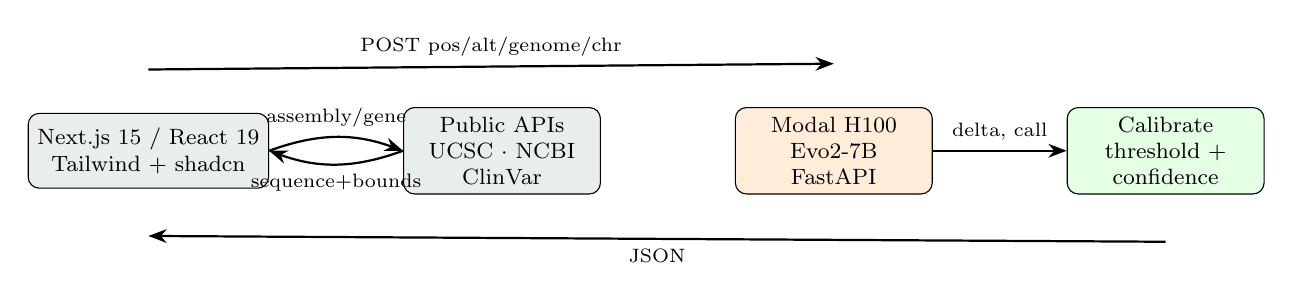
\begin{tikzpicture}[node distance=1.7cm,>=Stealth,
 box/.style={rectangle,draw,rounded corners,minimum width=2.5cm,minimum height=0.95cm,align=center,font=\footnotesize},
 small/.style={font=\scriptsize}]
\node[box,fill=evobg] (fe) {Next.js 15 / React 19\\Tailwind + shadcn};
\node[box,right=of fe,fill=evobg] (api) {Public APIs\\UCSC $\cdot$ NCBI\\ClinVar};
\node[box,right=of api,fill=orange!15] (mo) {Modal H100\\Evo2-7B\\FastAPI};
\node[box,right=of mo,fill=green!10] (cal) {Calibrate\\threshold +\\confidence};
\draw[->,thick,out=20,in=160] (fe.east) to node[small,above]{assembly/gene} (api.west);
\draw[->,thick,out=-160,in=-20] (api.west) to node[small,below]{sequence+bounds} (fe.east);
\draw[->,thick] ([yshift=0.55cm]fe.north) -- node[small,above]{POST pos/alt/genome/chr} ([yshift=0.55cm]mo.north);
\draw[->,thick] (mo.east) -- node[small,above]{delta, call} (cal.west);
\draw[->,thick] ([yshift=-0.6cm]cal.south) -- node[small,below]{JSON} ([yshift=-0.6cm]fe.south);
\end{tikzpicture}
\begin{itemize}\small
\item Browser never touches GPU. Weights stay warm on \texttt{hf\_cache} volume; \texttt{@enter} loads once, \texttt{scaledown\_window=120s}.
\end{itemize}
\end{frame}

% ---------- METHODOLOGY SCORING ----------
\begin{frame}{Methodology: Windowing and Scoring}
\begin{columns}[T]
\begin{column}{0.52\textwidth}
\small For 1-indexed position $p$, window $W{=}8192$:
\begin{equation*}
s{=}\max(0,p{-}1{-}W/2),\; e{=}\min(L,p{-}1{+}W/2{+}1)
\end{equation*}
Offset $r{=}p{-}1{-}s$, splice:
\begin{equation*}
w^{var}{=}w_{0:r}{+}\text{ALT}{+}w_{r+1:}
\end{equation*}
Score both, delta:
\begin{equation*}
\boxed{\Delta = S(w^{var})-S(w^{ref})}
\end{equation*}
\small Negative $\Delta$ = alternate less plausible. Ref windows deduplicated ($\sim$1/3 fewer calls).
\end{column}
\begin{column}{0.48\textwidth}
\centering
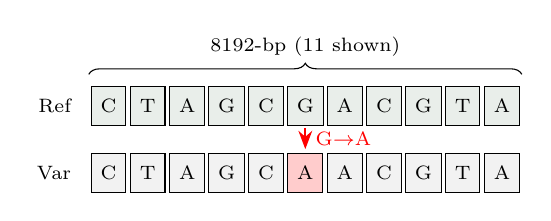
\begin{tikzpicture}[>=Stealth,font=\scriptsize,
 base/.style={rectangle,draw,minimum width=0.42cm,minimum height=0.5cm,align=center}]
\foreach \i/\b in {1/C,2/T,3/A,4/G,5/C,6/G,7/A,8/C,9/G,10/T,11/A} {\node[base,fill=evobg] at (\i*0.5,0) {\b};}
\node[base,fill=red!20] at (6*0.5,-0.85) {A};
\foreach \i/\b in {1/C,2/T,3/A,4/G,5/C,7/A,8/C,9/G,10/T,11/A} {\node[base,fill=gray!10] at (\i*0.5,-0.85) {\b};}
\node[anchor=east] at (1*0.5-0.35,0) {Ref};
\node[anchor=east] at (1*0.5-0.35,-0.85) {Var};
\draw[decorate,decoration={brace,amplitude=4pt}] (1*0.5-0.25,0.4) -- (11*0.5+0.25,0.4) node[midway,above=3pt]{8192-bp (11 shown)};
\draw[->,thick,red] (6*0.5,-0.28) -- (6*0.5,-0.55) node[midway,right]{G$\rightarrow$A};
\end{tikzpicture}
\end{column}
\end{columns}
\end{frame}

% ---------- CALIBRATION ----------
\begin{frame}{Methodology: Threshold, Confidence, Position}
\begin{columns}[T]
\begin{column}{0.5\textwidth}
\small ROC on $-\Delta$: $J{=}\max(\text{TPR}{-}\text{FPR})$, $\tau{=}-t^{\star}\approx -0.00092$.
\begin{equation*}
\text{call}=\begin{cases}\text{Pathogenic},&\Delta<\tau\\\text{Benign},&\text{else}\end{cases}
\end{equation*}
\begin{equation*}
\boxed{\text{conf}=\min\left(1,\frac{|\Delta-\tau|}{\sigma_{class}}\right)}
\end{equation*}
\small $\sigma_{LOF}{\approx}0.00151$, $\sigma_{FUNC}{\approx}0.00090$. RoPE: positions are angles, attention sees relative offset --- enables 8k$\rightarrow$1M.
\end{column}
\begin{column}{0.5\textwidth}
\centering
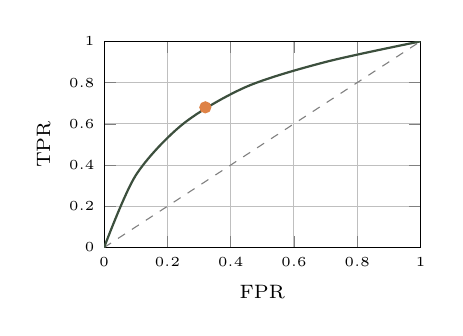
\begin{tikzpicture}
\begin{axis}[width=5.6cm,height=4.2cm,grid=major,xlabel={FPR},ylabel={TPR},xmin=0,xmax=1,ymin=0,ymax=1,tick label style={font=\tiny},label style={font=\scriptsize}]
\addplot[dashed,gray] coordinates {(0,0) (1,1)};
\addplot[thick,evogreen,smooth] coordinates {(0,0) (0.1,0.35) (0.25,0.6) (0.45,0.78) (0.7,0.9) (1,1)};
\addplot[only marks,evoorange,mark=*] coordinates {(0.32,0.68)};
\end{axis}
\end{tikzpicture}
\end{column}
\end{columns}
\end{frame}

% ---------- IMPLEMENTATION ----------
\begin{frame}{Implementation: Frontend Flow}
\begin{columns}[T]
\begin{column}{0.45\textwidth}
\small Entirely client fetches:
\begin{enumerate}\small
\item UCSC assemblies $\rightarrow$ chromosomes
\item clinicaltables gene search / chromosome filter (10 max)
\item E-summary bounds + UCSC sequence (10k view cap)
\item ClinVar E-search + E-summary (20 max)
\item Modal POST $\rightarrow$ comparison modal
\end{enumerate}
\small Clicking a base prefills pos/ref.
\end{column}
\begin{column}{0.55\textwidth}
\centering
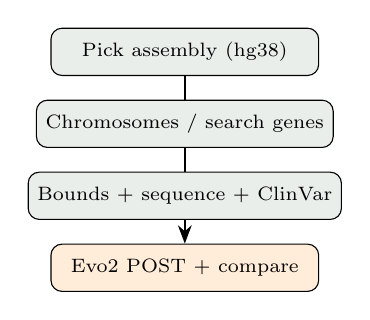
\begin{tikzpicture}[font=\scriptsize,>=Stealth,
 n/.style={rectangle,draw,rounded corners,minimum width=3.4cm,minimum height=0.6cm,align=center,fill=evobg}]
\node[n] (a) {Pick assembly (hg38)};
\node[n,below=0.3cm of a] (b) {Chromosomes / search genes};
\node[n,below=0.3cm of b] (c) {Bounds + sequence + ClinVar};
\node[n,below=0.3cm of c,fill=orange!15] (d) {Evo2 POST + compare};
\draw[->,thick] (a)--(b)--(c)--(d);
\end{tikzpicture}
\end{column}
\end{columns}
\end{frame}

\begin{frame}{Implementation: Backend (Modal H100)}
\begin{columns}[T]
\begin{column}{0.5\textwidth}
\begin{itemize}\small
\item Image: \texttt{cuda:12.6.3} + py3.12, torch 2.7 cu126, flash-attn 2.8, Evo2 pkg
\item Volume \texttt{hf\_cache} $\rightarrow$ \texttt{/root/.cache/huggingface}
\item \texttt{@modal.enter}: load \texttt{Evo2('evo2\_7b')} once
\item \texttt{@fastapi\_endpoint POST}: validate \texttt{VariantRequest}, fetch UCSC window, check bounds, score ref+var
\item \texttt{max\_containers=3, retries=2}
\end{itemize}
\end{column}
\begin{column}{0.5\textwidth}
\small Tech stack:
\begin{table}\scriptsize
\begin{tabular}{@{}ll@{}}
\toprule
Layer & Choice \\
\midrule
Model & Evo2-7B, StripedHyena2 \\
Serve & Modal H100, FastAPI \\
Compute & PyTorch, FlashAttention-2 \\
Web & Next.js 15, React 19, Tailwind \\
Data & UCSC, NCBI, ClinVar \\
Analysis & sklearn ROC, seaborn \\
\bottomrule
\end{tabular}
\end{table}
\end{column}
\end{columns}
\end{frame}

\begin{frame}{Implementation Progress}
\begin{table}\small
\begin{tabular}{@{}lll@{}}
\toprule
Area & Done & In progress \\
\midrule
Genome browse & Assembly/chr/gene/sequence/ClinVar & Pagination beyond 20 \\
Scoring & 8k window, dedup, $\Delta$, thr+conf & Indel support (SNV-only now) \\
Calibration & BRCA1-500, ROC/Youden, plot & Per-gene recal (hg19 thr on hg38) \\
Deploy & Modal H100 live, Next.js dev & Vercel config, API auth \\
\bottomrule
\end{tabular}
\end{table}
\end{frame}

% ---------- RESULTS ----------
\begin{frame}{Results: BRCA1 Separation}
\begin{columns}[T]
\begin{column}{0.5\textwidth}
\centering
\begin{tikzpicture}
\begin{axis}[width=5.8cm,height=4.0cm,boxplot/draw direction=y,xlabel={$\Delta$},ylabel={class},ytick={1,2},yticklabels={FUNC/INT,LOF},xmin=-0.008,xmax=0.004,tick label style={font=\tiny}]
\addplot+[boxplot,fill=gray!20] coordinates {(-0.001,1) (-0.0002,1) (0.0005,1) (0.001,1) (0.0002,1)};
\addplot+[boxplot,fill=red!20] coordinates {(-0.004,2) (-0.002,2) (-0.0012,2) (-0.0003,2) (-0.0015,2)};
\draw[dashed] (axis cs:-0.00092,0.8) -- (axis cs:-0.00092,2.2) node[above,font=\tiny]{$\tau$};
\end{axis}
\end{tikzpicture}
\end{column}
\begin{column}{0.5\textwidth}
\begin{itemize}\small
\item LOF mass left of $\tau$, functional right
\item AUROC $\approx$ 0.73 on 500 BRCA1 SNVs (zero-shot, no fine-tune)
\item Consistent with Evo2 report trend
\item Live case: \texttt{hg38 chr17:43119628 G} $\rightarrow$ JSON with delta/prediction/confidence next to ClinVar
\end{itemize}
\end{column}
\end{columns}
\end{frame}

\begin{frame}{Limits and Next Steps}
\begin{columns}[T]
\begin{column}{0.5\textwidth}
\textbf{Limits (honest):}
\begin{itemize}\small
\item SNV-only; title-regex breaks on dels
\item hg19-derived $\tau$ applied to hg38/other genes
\item Public API caps; fragile ClinVar parsing
\end{itemize}
\end{column}
\begin{column}{0.5\textwidth}
\textbf{Next:}
\begin{itemize}\small
\item Deletion/insertion splice + validation
\item Per-gene recal + batch endpoint
\item Auth on FastAPI, Vercel deploy, theme tokens
\end{itemize}
\end{column}
\end{columns}
\end{frame}

\begin{frame}[allowframebreaks]{References}
\tiny
\begin{enumerate}
\item G.~Brixi et al., Genome modeling and design with Evo2, bioRxiv 2025.02.18.638918, 2025.
\item E.~Nguyen et al., Sequence modeling with Evo, Science 386, 2024.
\item J.~Cheng et al., AlphaMissense, Science 381, 2023.
\item Z.~Lin et al., ESM-2, Science 379, 2023.
\item H.~Dalla-Torre et al., Nucleotide Transformer, Nat.\ Methods, 2023.
\item M.~Poli et al., Hyena Hierarchy, ICML 2023.
\item J.~Su et al., RoFormer (RoPE), Neurocomputing 568, 2024.
\item T.~Dao, FlashAttention-2, 2023.
\item Z.~Avsec et al., Enformer, Nat.\ Methods 18, 2021.
\item J.~Linder et al., Borzoi, Nat.\ Genet.\ 2023.
\item C.~Lee et al., UCSC Genome Browser, NAR 50, 2022.
\item M.~Landrum et al., ClinVar, NAR 42, 2014; update 2024.
\item S.~Richards et al., ACMG guidelines, Genet.\ Med.\ 17, 2015.
\item M.~Kircher et al., CADD, Nat.\ Genet.\ 46, 2014.
\item Modal docs; Next.js docs; FastAPI docs, 2024.
\end{enumerate}
\end{frame}

\begin{frame}
\centering
{\Large Thank you} \\[0.5em]
Questions? \\[0.5em]
{\small Repo: variant-analysis-evo2 \quad Demo: hg38 $\rightarrow$ BRCA1 $\rightarrow$ Analyze}
\end{frame}

\end{document}
